% Created 2016-08-17 Wed 14:38
\documentclass[tikz]{standalone}

\usepackage[utf8]{inputenc}
\usepackage[T1]{fontenc}

\usepackage{circledsteps}

\RequirePackage{xcolor}

%% HPI color definitions according to the design manual
% These do not exactly match the RGB values used in the Powerpoint slide master due to unknown reasons
\definecolor{hpiyellow}{RGB}{246,168,0}
\definecolor{hpiorange}{RGB}{221,97,8}
\definecolor{hpired}{RGB}{177,6,58}
\definecolor{hpigray}{RGB}{90,96,101}
\definecolor{hpiblue}{RGB}{0,122,158}


\renewcommand{\sfdefault}{neosans}
% Different font weights for neosans
\newcommand{\textl}[1]{{\fontseries{l}\selectfont #1}} % light
\newcommand{\textm}[1]{{\fontseries{m}\selectfont #1}} % medium, same as default weight
\newcommand{\textsb}[1]{{\fontseries{sb}\selectfont #1}} % semibold
\newcommand{\textmb}[1]{{\fontseries{mb}\selectfont #1}} % bold, same as \textbf
\newcommand{\texteb}[1]{{\fontseries{eb}\selectfont #1}} % extra bold
\newcommand{\textub}[1]{{\fontseries{ub}\selectfont #1}} % ultra bold

\tikzset{every picture/.style={/utils/exec={\sffamily}}}
\tikzset{flipflop RSflanke/.style={
  flipflop,
  flipflop def={t1=S, t2=C, c2=1, t3=R, t6=Q, t4={\ctikztextnot{Q}}}
}}


\tikzset{
  mechanicalSwitch/.pic={
    \coordinate (-inUp) at (135:2); 
    \coordinate (-inDown) at (235:2);
    \coordinate (-out) at (2,0);
    \coordinate (-center) at (0,0);
    
    \draw (0,0) circle [radius = 2cm];
    \draw [fill=gray!20] (0,0) circle [radius = 0.2cm];

    \draw (0, 0) -- (2, 0);
    \draw (135:.8) -- (135:2); 
    \draw (225:.8) -- (225:2); 

    \draw [fill=gray!20] (2, 0) circle [radius=0.05cm]; 
    \draw [fill=gray!20] (135:2) circle [radius=0.05cm]; 
    \draw [fill=gray!20] (225:2) circle [radius=0.05cm]; 

    
    \draw [thick] (0,0) -- (175:1.5); 

    \draw [dashed, <->, domain=135:225] plot ({cos(\x)}, {sin(\x)}); 
  },
  mechanicalSwitchClosed/.pic={
    \coordinate (-inUp) at (135:2); 
    \coordinate (-inDown) at (255:2);
    \coordinate (-out) at (2,0);
    \coordinate (-center) at (0,0);
    \draw (0,0) circle [radius = 2cm];
    \draw [fill=gray!20] (0,0) circle [radius = 0.2cm];

    \draw (0, 0) -- (2, 0);
    \draw (135:.8) -- (135:2); 
    \draw (225:.8) -- (225:2); 

    \draw [fill=gray!20] (2, 0) circle [radius=0.05cm]; 
    \draw [fill=gray!20] (135:2) circle [radius=0.05cm]; 
    \draw [fill=gray!20] (225:2) circle [radius=0.05cm]; 

    
    \draw [thick] (0,0) -- (135:2); 

    \draw [dashed, <->, domain=135:225] plot ({cos(\x)}, {sin(\x)}); 
  }
}


\usetikzlibrary{calc}
\usetikzlibrary{positioning}


\usepackage{../../templates/moeptikz}
\usepackage{bytefield}
\usetikzlibrary{backgrounds,fit,shapes.symbols}
\begin{document}

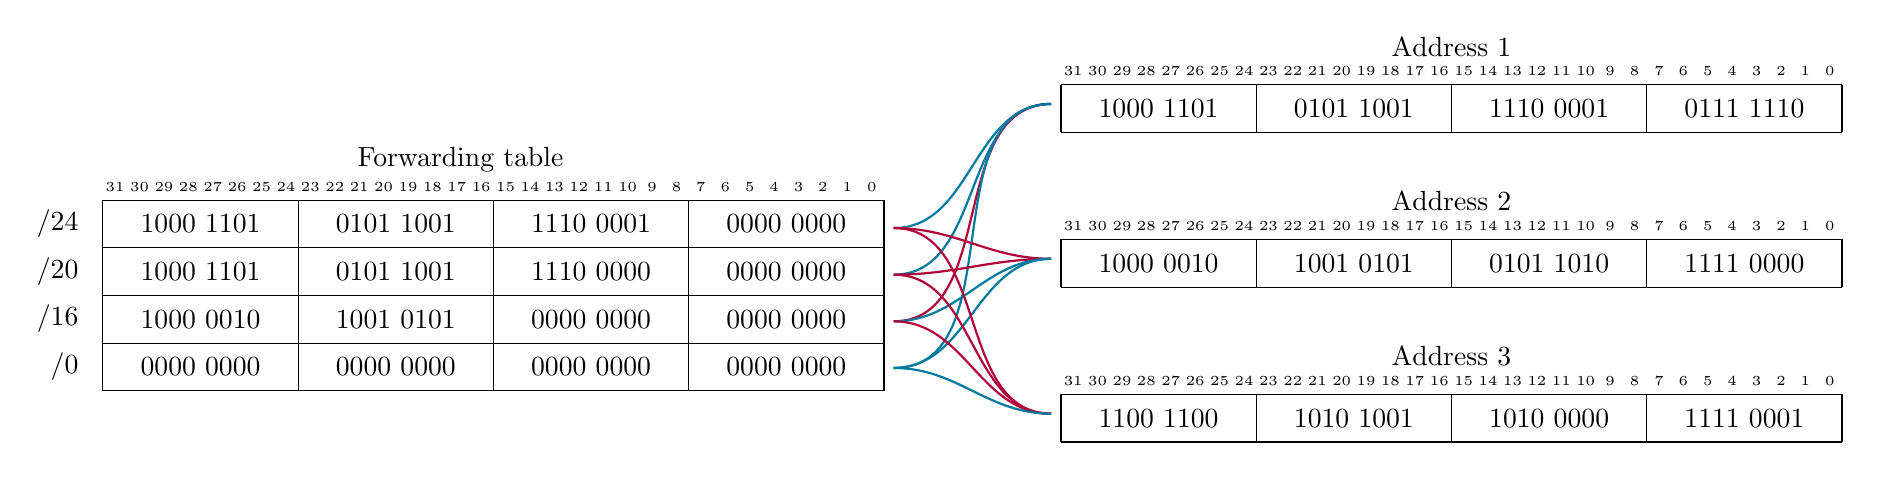
\begin{tikzpicture}
  \label{page:routing:prefix_matching}

  \node [label=above:Forwarding table] (rt)  {
    \begin{bytefield}[endianness=big]{32}
      \bitheader{0-31}\\
      \begin{leftwordgroup}[leftcurly=.]{/24}
        \bitbox{8}{1000 1101} 
        & \bitbox{8}{0101 1001}  
        & \bitbox{8}{1110 0001}
        & \bitbox{8}{0000 0000}
      \end{leftwordgroup}\\
      \begin{leftwordgroup}[leftcurly=.]{/20}
        \bitbox{8}{1000 1101} 
        & \bitbox{8}{0101 1001}  
        & \bitbox{8}{1110 0000}
        & \bitbox{8}{0000 0000}
      \end{leftwordgroup}\\
      \begin{leftwordgroup}[leftcurly=.]{/16}
        \bitbox{8}{1000 0010} 
        & \bitbox{8}{1001 0101}  
        & \bitbox{8}{0000 0000}
        & \bitbox{8}{0000 0000}
      \end{leftwordgroup}\\
      \begin{leftwordgroup}[leftcurly=.]{/0}
        \bitbox{8}{0000 0000} 
        & \bitbox{8}{0000 0000}  
        & \bitbox{8}{0000 0000}
        & \bitbox{8}{0000 0000}
      \end{leftwordgroup}\\
    \end{bytefield}
  };

  \foreach \i in {1,...,4} {
    \coordinate (pre\i) at ($([yshift=-0cm]rt.north east)!\i/4!([yshift=0.8cm]rt.south east)$);
    % \node [red] at (pre\i) {X}; 
  }


  \node [above right=0.5cm and 2cm of rt,label=above:Address 1] (p1) {
    \begin{bytefield}[endianness=big]{32}
      \bitheader{0-31}\\
      \bitbox{8}{1000 1101} 
      & \bitbox{8}{0101 1001}  
      & \bitbox{8}{1110 0001}
      & \bitbox{8}{0111 1110}
    \end{bytefield}
  };

  \foreach \i/\m in {1/hpiblue,2/hpiblue,3/hpired,4/hpiblue} {
    \draw [thick,\m] (p1.west) to [out=180,in=0] (pre\i); 
  }


  \node [below=of p1,label=above:Address 2] (p2) {
    \begin{bytefield}[endianness=big]{32}
      \bitheader{0-31}\\
      \bitbox{8}{1000 0010} 
      & \bitbox{8}{1001 0101}  
      & \bitbox{8}{0101 1010}
      & \bitbox{8}{1111 0000}
    \end{bytefield}
  };

  \foreach \i/\m in {1/hpired,2/hpired,3/hpiblue,4/hpiblue} {
    \draw [thick,\m] (p2.west) to [out=180,in=0] (pre\i); 
  }


  \node [below=of p2,label=above:Address 3] (p3) {
    \begin{bytefield}[endianness=big]{32}
      \bitheader{0-31}\\
      \bitbox{8}{1100 1100} 
      & \bitbox{8}{1010 1001}  
      & \bitbox{8}{1010 0000}
      & \bitbox{8}{1111 0001}
    \end{bytefield}
  };


  \foreach \i/\m in {1/hpired,2/hpired,3/hpired,4/hpiblue} {
    \draw [thick,\m] (p3.west) to [out=180,in=0] (pre\i); 
  }

\end{tikzpicture}


\newcommand{\subnetting}[0]{  \node [router, label=below:Router 1] (r1) {};
  \node [above right=0.1cm of r1.east] (r1Prefix) {200.23.16.0/20};

  \node [router, above left=1cm and 4.5cm of r1,label=below:Router 1a] (r1a) {}; 
  \node [router, below=of r1a,label=below:Router 1b] (r1b) {}; 
  \node [router, below=of r1b,label=below:Router 1h] (r1h) {};

  \draw (r1a.east) -- ++ (3,0) node [above] {200.23.16.0/23\\(\dots .0001 000.0)} |- (r1.west); 
  \draw (r1b.east) -- ++ (2,0) node [above] {200.23.18.0/23\\(\dots .0001 010.0)} |- (r1.west); 
}

\begin{tikzpicture}[every node/.style={align=center}]
  \label{page:routing:ip:subnetting}

  \subnetting
  \draw (r1h.east) -- ++ (3,0) node [below] {200.23.30.0/23\\(\dots .0001 1110.0)} |- (r1.west); 
  
\end{tikzpicture}

\begin{tikzpicture}[every node/.style={align=center}]
  \label{page:routing:ip:internet_prefixes}

  \subnetting
  \draw (r1h.east) -- ++ (3,0) node [below] {200.23.30.0/23\\(\dots .0001 1110.0)} |- (r1.west); 

  \node [router, below=4cm of r1, label=below:Router 2]  (r2) {};
  \node [cloud, draw, scale=3, left=of r2] (n2) {};
  \node [below right=0.1cm of r2.east] (r2Prefxi) {199.31.0.0/16};
  \draw (r2) -- (n2); 
  
  \node [cloud, draw, scale=2, below right=1cm and 2cm of r1Prefix] (internet) {Internet};

  \node [router, below right=0.4cm of internet.west, label=below:Router 3] (ri) {}; 
  
  \draw [very thick] (r1.east) -- (internet.150) -- (ri); 
  \draw [very thick] (r2.east) -- (internet.240) -- (ri); 
  % -- (r2.east); 
\end{tikzpicture}


\begin{tikzpicture}[every node/.style={align=center}]
  \label{page:routing:ip:changed_prefixes}

  \subnetting

  \node [router, below=4cm of r1, label=below:Router 2]  (r2) {};
  \node [cloud, draw, scale=3, left=of r2] (n2) {};
  \node [below right=0.4cm of r2.east] (r2Prefxi) {199.31.0.0/16\\200.23.30.0/23
  };
  \draw (r2) -- (n2); 


  \draw (r1h.east) -- ++ (3,0) node [above] {200.23.30.0/23\\(\dots .0001 1110.0)} -| (r2.north); 

  
  \node [cloud, draw, scale=2, below right=1cm and 2cm of r1Prefix] (internet) {Internet};

  \node [router, below right=0.4cm of internet.west, label=below:Router 3] (ri) {}; 
  
  \draw [very thick] (r1.east) -- (internet.150) -- (ri); 
  \draw [very thick] (r2.east) -- (internet.240) -- (ri); 
  % -- (r2.east); 
\end{tikzpicture}



% -----------------
% complex scenario for ARP

\begin{tikzpicture}
  \node [client, label={[align=center]below:Client\\IP}] (client) {}; 
  \node [switch, right=of client, label={[align=center]below:Switch A}] (swA) {};
  \node [router, right=of swA, label={[align=center]below:Router 1}] (r1) {};
  \node [switch, right=of r1, label={[align=center]below:Switch B}] (swB) {};
  \node [router, right=of swB, label={[align=center]below:Router 2}] (r2) {};
  \node [switch, right=of r2, label={[align=center]below:Switch C}] (swC) {};
  \node [server, right=of swC, label={[align=center]below:Server}] (server) {};

  \draw (client) -- (swA) -- (r1) -- (swB) -- (r2) -- (swC) -- (server);

  \begin{scope}[on background layer]
    \node [fill=hpiyellow!10, fit=(client)(swA)(r1.west)] {}; 
    \node [fill=hpiblue!10, fit=(r1.east)(swB)(r2.west)] {}; 
    \node [fill=hpiorange!10, fit=(r2.east)(swC)(server)] {}; 
  \end{scope}
  
  
\end{tikzpicture}



\end{document}